\chapter{Modular Anomaly Detection Framework}
\label{chapter:Chapter 3}
\lhead{Chapter 3. \emph{Methods and Systems Developed}}

In this Chapter, we present the proposed Modular Anomaly Detection Framework. Firstly list the actual requirements that served as a blueprint for the developed Framework. This requirements were either defined by Maritime Officer Experts under the MARISA project, or from limitations from the Data either from the  

Second we show the proposed Modular Anomaly Detection Framework, as shown in Fig. XX. And in the following sections we provide a overall explanation of each module functionality. 

by describing the overall view of the proposed Modular Framework, Secondly we provide a detailed explanation of each Module and the methods used for each Module. 


\section{Anomaly Definition}
An Anomaly can have numerous interpretations depending on the context in which is found, but it can be generally defined as Data that stand out when contrasted to other Data.

Nowadays Vessel Anomaly Detection is solely done by Human Maritime Experts, with every Maritime Security Agency assuring the coastal surveillance of their territory, by assessing possible threats, and identifying abnormal behaviour. 
%The identified abnormal Vessel behaviour is then further investigated by Maritime Authorities, which can lead to fines or even criminal charges against the Vessel crew. 
The problem of this current methodology for Anomaly Detection, is that is extremely inefficient. Human analysis only allows a limited number of Vessels that can be analyzed. This problem is aggravated as the number of Vessel at seas is increasing every year in a exponential rate. 

This creates a typical situation for the use of Machine Learning models to aid the necessities of Maritime Experts.
%, in the field of Maritime Anomaly Detection.
Although, formalizing an Vessel Anomalous Behavior is extremely difficult, as it is not clear what is Anomalous in the when only analyzing the Maritime data, and there is no available historical Anomalous Data-Set, to the best of our knowledge.

To solve this problem of the defining Vessel Abnormal Behaviour, Expert Knowledge from Maritime Experts was accessed under the MARISA project. Maritime Experts in order to define Anomalies which could be formalized, provided a list of Vessels Anomalies which behaviour. firstly a list of  



%It is impossible to define Anomalous, when only   

%any Vessel Anomaly can be caused by a undetermined number of factors,      . 

Thus, the context and causes of every Anomaly needs defined by Maritime Experts. Thus, in order to surpass the problem of the definition of an Anomaly; Expert Knowledge from Maritime Experts was accessed under the MARISA project. Maritime Experts defined, firstly a list of  

\section{Framework Requirements}
\label{section: Framework Requirements}
In order to develop a framework that will addresses the real demands of Maritime Officers, we surveyed the only agents that could significantly insight Maritime Officers under the MARISA project. in order to fully understand the demands for a Framework for Maritime Anomaly Detection.
This being said, for the defined requirements we categorized them into three main classes:

\begin{description}
\item[Anomalies Detection Requirements] Having the concept of Behavioural Vessel Anomaly listed by Maritime Officers is the most reliable way to grasp the concept of Anomaly at Seas. Therefore, Maritime Officers defined a list of Anomalies, for which we developed methods to detect those anomalies. 
\begin{enumerate}[label=(\subscript{AR}{{\arabic*}})]
    \item
    Detect Abnormal changes of (more than a configurable value) Direction.
    \item
    Detect Vessels disappearance from sensor coverage for more than a configurable Time period.
    \item
    Detect when the observed Vessel Navigational Status is not consistent with the reported Vessel Kinematic features.
    \item
    Detect when Vessels report a geographical and time incompatibility.
    \item
    Detect when two or more Vessels are approaching close to each other.
\end{enumerate}









%Being the one truly viable method to define of the methods we used to detect anomalies in the data, sequence of features is transformed into a feature vector, then convectional classification methods are applied. Feature selection represents is an important task for this method of classification.

\item [Functional Requirements] As the developed Framework was implemented so it could be used by Maritime Authorities, it was completely mandatory that the Framework could be not only deployed in different environment, but also completely modular and scallable; as different Maritime Authorities have different requirements. 
not controlled by us.

\item [Data Requirements] This requirements, were the class of requirements were not so obvious to classify. Any Framework that deals with Maritime data, is certain that it needs to be implemented so it can handle really high workflows of data, due to the increasing volume of Vessels at Seas. Although, Maritime is represented by different types of data from Meteo data to AIS data to even Fishing logs data, which come in different structures, or even with no structure at all.
\end{description}

\todo[inline]{NEED A TABLE OR SOMETHING WITH THE ACTUAL REQUIREMENTS}


\section{Proposed Framework}
In order to develop a Framework capable of addressing the requirements defined, above in \ref{section: Framework Requirements}, we propose a Modular Vessel Anomaly Detection Framework, able to ingest data from different feeds in real-time data, construct a Data-Base for Vessels Trajectories in a unsupervised manner, and detect different Anomalies over either real-time incoming data or stored Vessels Trajectories; as it is represented in \ref{fig:Framework}.

We provide a Modular Framework, as there are no inputs or outputs absolute standards nor defined requirements for any System for Anomaly Detection on the Maritime domain, so by providing a configurable and specially not static Framework, we provide the flexibility for providing the same Framework configured for different scenarios or even different National Maritime Authorities.

as the requirements for one so by defining a Framework allows a flexible configuration from either types of Anomalies, system, allows a easier adoption of these services by Maritime end users. 

on a Lambda Architecture, and having the Apache Ecosystem. composed from four main modules, as shown in Fig. XX ...

\begin{figure}[H]
	\centering
	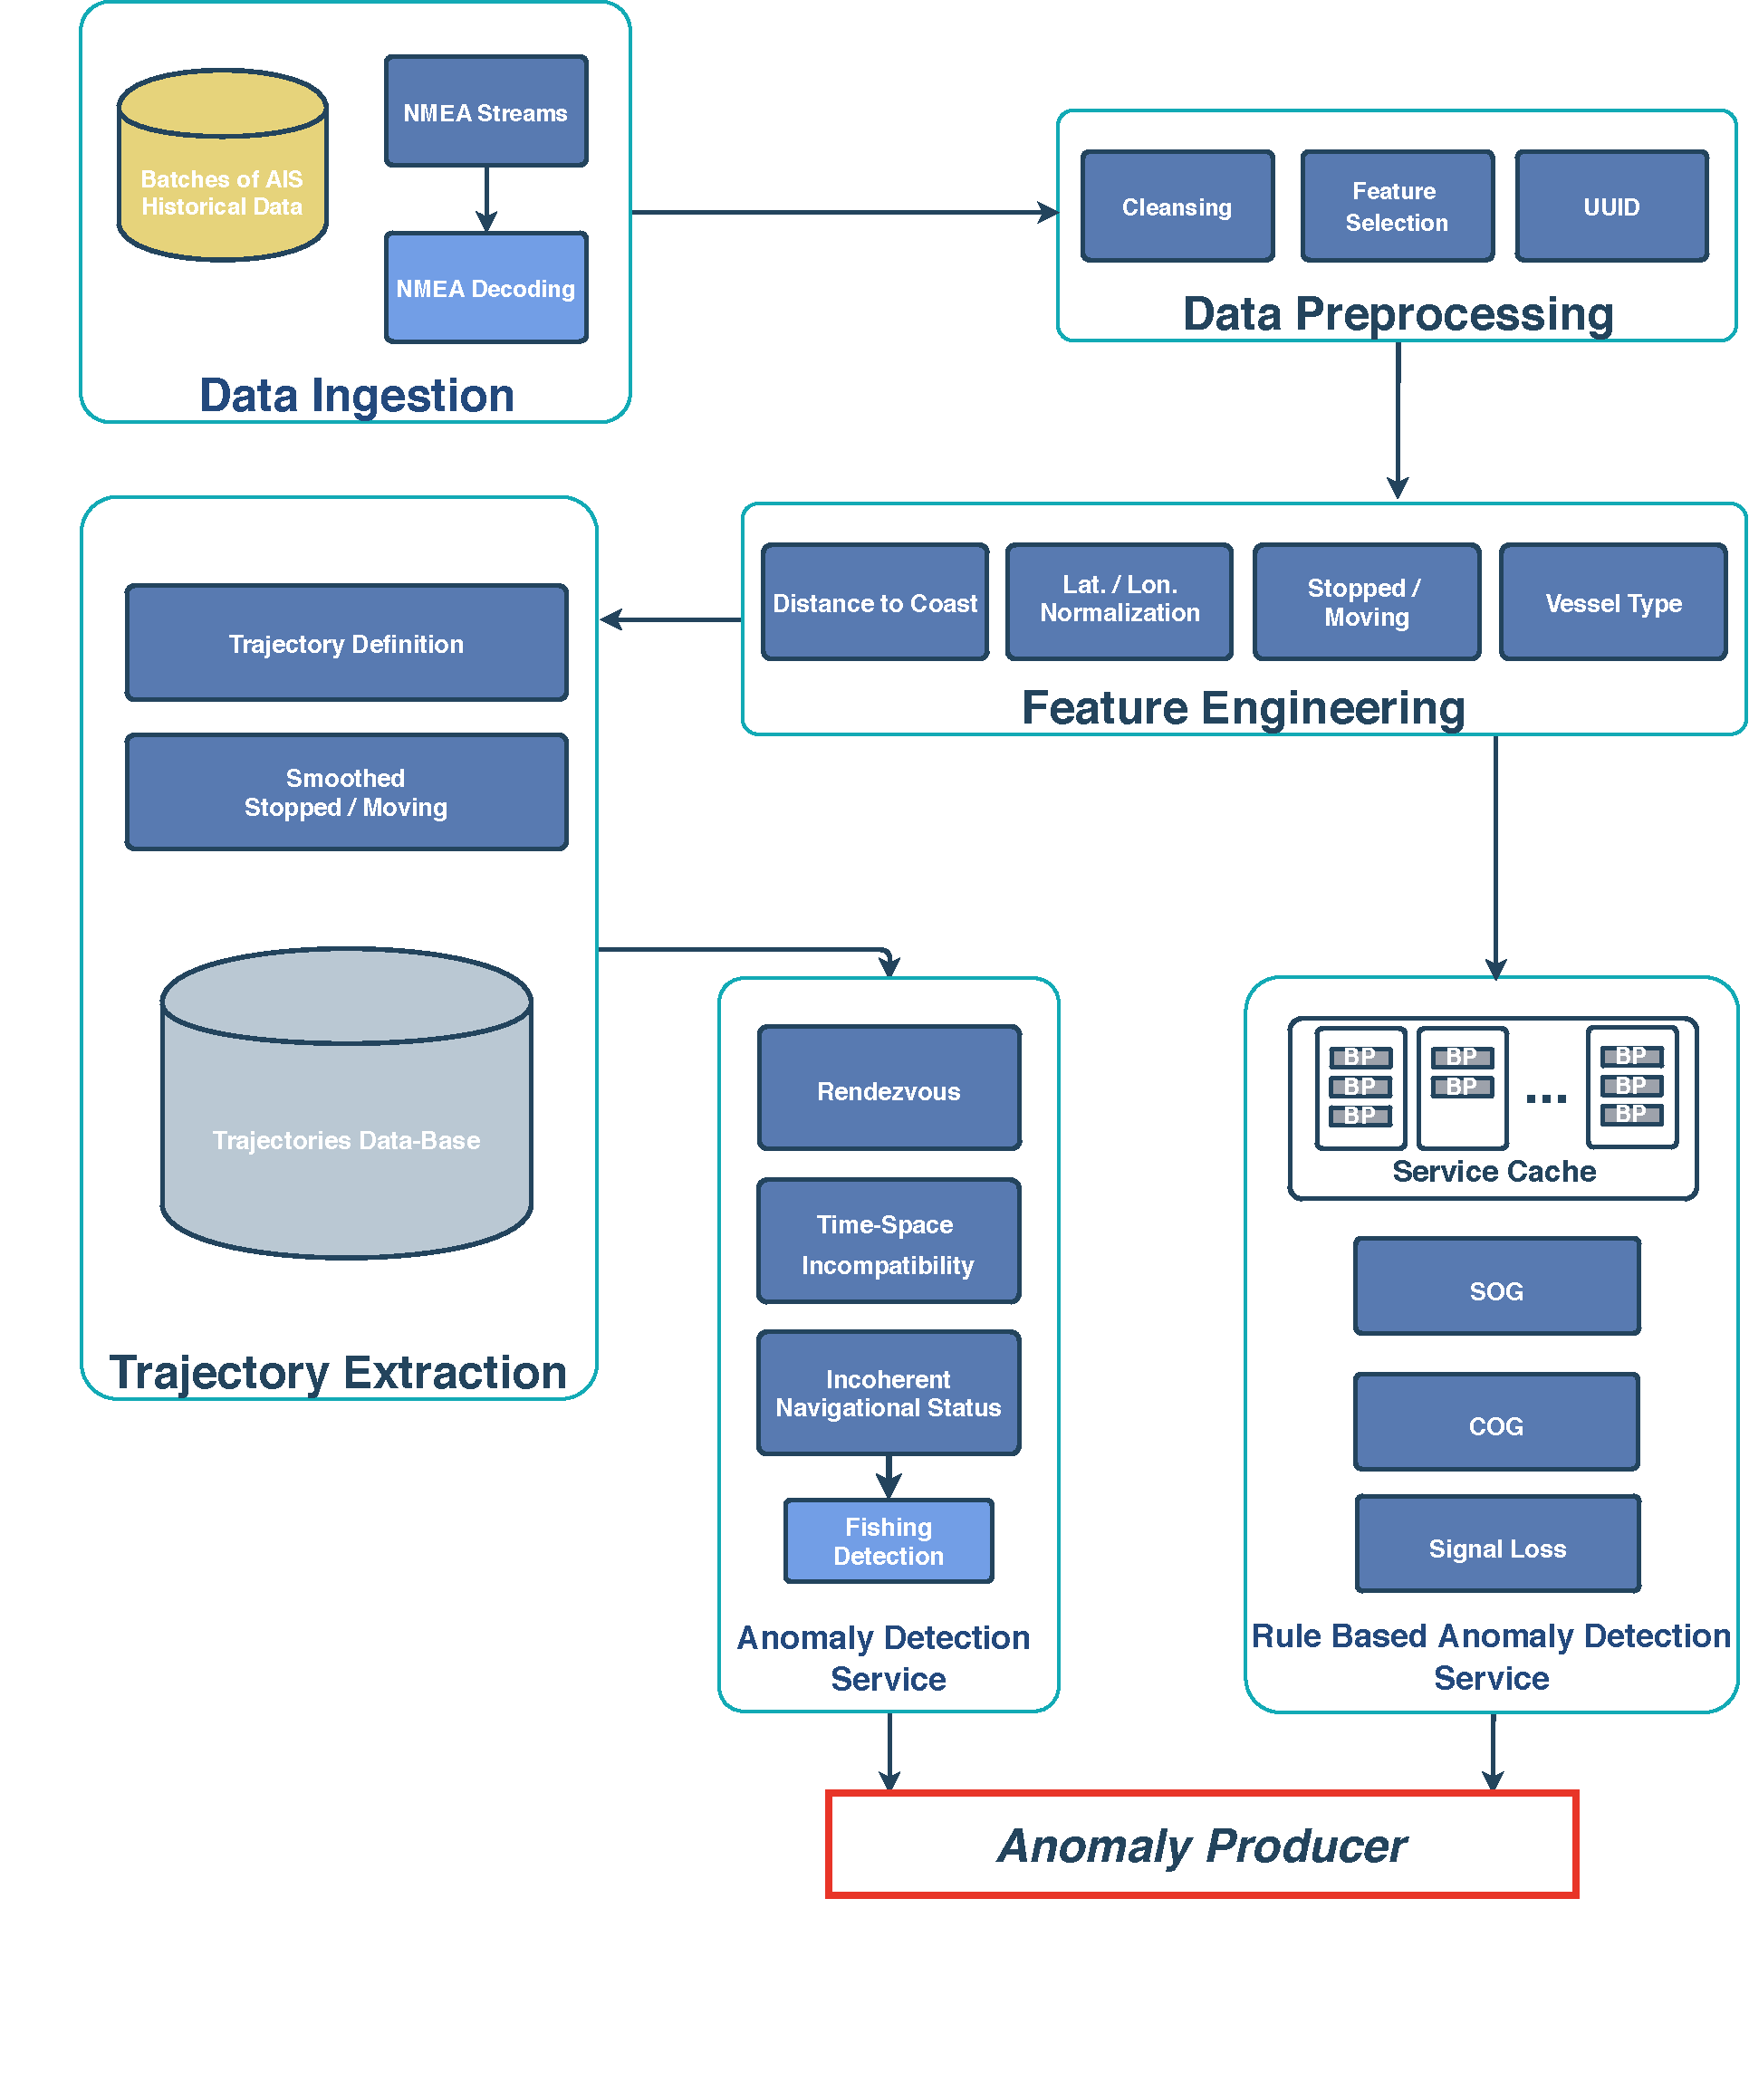
\includegraphics[scale = .37]{figures/Ch3/Framework.pdf}
    \caption{Proposed Beta Framework \todo[inline]{NEEDS MORE DETAIL THIS IMAGE}.}
    \label{fig:Framework}
\end{figure}

In the following subsections, we discuss each module: Data Fusion, Vessel T Extraction, Anomaly Detection and Reporting...

\subsection{Data Ingestion}
Data Ingestion Module, represents the Data input for the developed Framework. AIS data was the most representative data type used for this work, as it showcases the actual instantaneous Vessel information.
Although, used AIS data for this work came in two really distinct formats: It came either in \textbf{Historical Batches} representing Historical sets of Data, or real \textbf{NMEA AIS Streams}, which represent real, real-time data. For both formats of AIS data, the framework is scallable, and able to Ingest one or multiple feeds / sources of AIS data.

AIS Historical Data-Sets, can be found in open-access repositories, although Historical AIS Data providers cap the frequency of the messages transitions. This drastically reduces the number of transmitted messages, but also reduces the overall detail of the Data, as lower transmissions rates produce a less certainty of the movement presented by each Vessel. Which, for most general uses of AIS (e.g. managing a fleet, estimations of time of arrival ...), transmissions rates of 3 Seconds vs 30 Seconds, do not provide any information gain, as Vessel kinematics tend to not change abruptly in short periods of time. 

Via the MARISA project, we received AIS live feeds from Antennas all around the European coast. This Antennas receive the Vessels transmissions broadcast via AIS, till normally a range of 20 Nautical Miles of the shore and depending on the live feed provider, AIS messages can be received in rates up to 30 Messages per Minute per Vessel. This type of incoming Data Streams represents the Real scenario, in which the Framework will be tested. Real live streams of AIS data, are received via TCP stream in NMEA format which in order to be represented as AIS messages required to be decoded, which is described in the subsection under.


\subsubsection{NMEA Decoding}
National Marine Electronics Association (NMEA) is a standard communication protocol used by Maritime Sensors such as Accelerometer, Giroscope, GPS receivers, etc.
NMEA encapsulates the information from the different Vessel sensors, and broadcasts this information

being the standard it is the protocol that encapsulates the AIS information, broadcasted by AIS-equipped Vessels. 

\begin{figure}[H]
	\centering
	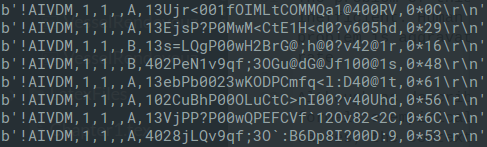
\includegraphics[scale = .5]{figures/Ch3/NMEAexample.png}
    \caption{Snapshot of raw AIS data in NMEA format.}
    \label{fig:NMEAexample}
\end{figure}

\todo[inline]{TODO SAME AS IN TOP ITS BS}

Via the project, we had access to multiple live NMEA feeds, as a way to not only validate our developed methods with live feeds of Nautical data, but also to produce methods that were capable of handling the scale of data that is produced by National feeds.

The use of real data comes with many challenges, as it is mandatory to decode sort and store this data in order to de accessed as a viable source of data; a snapshot of a example of a NMEA feed can be found in Figure \ref{fig:NMEAexample}. 

\todo[inline]{this might go to chap4}

AIS-Receiving stations receive the broadcast AIS information from numerous AIS-equipped Vessels simultaneously. Normally, AIS-Receiving stations are antennas located along the coast line in high grounds, the reception range of these antennas vary, mainly depending on distance to shore, the elevation in which the antenna is located, and the antenna type itself.

Although, the distance in which Stations are capable of receiving AIS messages presents a problem to the Data, as reception ranges vary from 15 Nautical Miles to 50 Nautical Miles, which creates the problem of 

\begin{enumerate}
\item Duplication of Reception:  With the variation of reception ranges, it frequently occurs that multiple stations, receive the same AIS Message

\todo[inline]{THIS BRINGS TO THE PROBLEM OF MULTIPLE ANTHENAS RECEIVING THE SAME FEED... disse que havia dois problemas}

\end{enumerate}

%\subsection{Data Storage}
%With NMEA streams producing enormous workflows of data, the storage of becomes a problem for the developed Framework, as it must not only decode and process the NMEA feeds but also store the decoded messages, in a "very fast" and scalable way.

%Thus, and as requirement of the MARISA project was to use Apache Spark [REF FOR APACHE SPARK] modules for data-ingestion and pre-processing, we decided to use Apache Cassandra as the Data-Storage for the proposed framework.

\subsection{Data Pre-processing}
The Data Pre-processing module, is the first step of Data Wrangling in our Framework, the motive for this module is to clean, transform and normalize, the AIS data.
% either from the different Sources of Historical AIS data or the decoded AIS NMEA live feeds, which come from the Data Ingestion Module.  

As described in Section \ref{subsection: chp2_AIS},  AIS presents a large amount of different features, which can be used for different problems. Selection the correct features that better describe the Vessels Behaviour,  requires a pre-conceived knowledge of Vessels dynamics which is gained with the experience on the Maritime Domain. 

%and estimating the real use-fullness of each feature, thus selecting the correct features that better describe the Vessels Behaviour,  requires a pre-conceived knowledge of Vessels dynamics that is gained with the experience on the Maritime Domain. 

Thus for this Framework, the choice of most suitable features that represent a Vessels movement was based on the literature and with the help of Maritime Knowledge Expert. Which lead to the choice of the features that represent the Vessels Kinematics.

At this step we correct data incompatibilities based on the information that standardizes this data, this is, as the reported AIS data corresponds to the Vessels Positional and Kinematic data it is assured that the features reported should come in a defined range of values as it is represented in Section\ref{section: Data Analysis}. Values not in this range are considered errors in the data. 

\todo[inline]{STANDART FEATURE VALUES TABLE HERE OR IN NEXT...}


\subsection{Feature Engineering}
Feature Engineering presents a crucial step for any machine learning project, as selecting the right features to represent the data, directly influences any result generated by the Anomaly Detection Modules.  




We further enrich our features in two ways, firstly by analyzing each AIS message as a single point in Time and calculating additional distances, such as distance to Shore and distance to the most near Port.

each point in t the represented features of each message by by doing a point based analysis, in which we considered the information of  

by normalizing the Latitude and Longitude features of each position, calculating the Distance to Shore and the kinematic features that represent the instantaneous move-state of the Vessel. Every calculation is done a priory, thus enhancing the performance and reliability of the Anomaly Detection Modules, which are explained in detail in section \todo{REF TO SECTION!}

\subsection{Vessel Trajectory Extraction}
Vessel Trajectory Extraction module, handles the definition, storage and updating of new Vessels AIS Messages into defined Trajectories.
By analyzing Trajectories, the reported AIS messages stop being represented as single points in Time, and start representing the aggregation of single AIS messages in a specific time-span, which allows a behaviour analysis based on the past trajectory of the Vessel. Although, in order to analyze a Trajectory, it is important to represent each Trajectory in a optimal manner, with no information loss, Trajectory Representation methods are presented in Section XX.  

As mentioned above, this module handles the storage of the Vessels trajectories, which requires a  

\todo[inline]{This might go to Data prepossessing.}
Furthermore, when dealing with real Maritime data (and specially when working with real Maritime Authorities) it is extremely important to have a traceback Data, from which we can justify the detection of the generated Anomalies for this we keep an historical 
increases complexity, 


which we consider as Vessel Trajectory. 

Behaviour analysis based on the past historical Trajectory data. Analysis of Trajectories drastically increases the level of complexity, when compared to analysis points, thus it is required quick and efficient representation of a Trajectory.


of the modules, thus requiring a 

previous  and its behaviour for a determine Time span. By analysing   

Which increases the complexity of the analysis, but is also the 
Trajectory which will represent the   permits the analysis of a used points,   


in order to discovery new knowledge, it is important to 


\subsection{Anomaly Detection Service}
ADS (Anomaly Detection Service) Module, represents in our architecture the module to Anomaly Detection, which runs in batches of data, making it only able to run in effective time opposed real-time. ADS works by querying data from the historical Trajectory Data-Base, with a configurable set of parameters, which can be time restrictive(such as the 10 past Hours) and or from a Vessel specific set of Vessels. This data is then fed to our Anomaly Detection Service Module, which were implemented to detect :

the Vessels Rendezvous and the miss using of the AIS Navigational Status.
For the latter, we create a sub-method for the detection of Fishing Activities based on Vessels characteristics and Dynamics and the reported Navigational Status.

%Although, the developed Framework being completely Modular we provide the scallability optito implement new AD methods, in this module...

\subsection{Rule Based - Anomaly Detection Service}
RB-ADS(Rule Based - Anomaly Detection Service), opposed to the ADS module described above corresponds to a real-time module where Anomalies which can be defined by a set of rules are detected.
AIS Messages, coming from streams(NMEA streams for this work), are firstly Pre-processed in the Data Pre-processed module described above. Afterwards, in order for the RB-ADS be able to perform in real-time AD we defined a queuing cache system which creates a Queue of pre-processes messages of size $N$ for every single Vessel that we had received a message from. 
The queuing system allows a real-time calculation of the any Anomaly which can be defined by Rules, although for this work we focused on the detection of the detection    

\subsubsection{AIS Signal Loss}
\todo[inline]{NEED TO DO REQUIREMENTS TABLE}
Ships equipped with AIS are obliged to keep the AIS autonomously transmitting AIS messages. A way that ships illegally hide their position and possible what the ships is doing objectively, is by switching off the AIS, or finding ways to block the communications of the AIS transmitter with the coastal receivers.

This creates a problem in the maritime domain, has maritime authorities are constantly finding new ways to discover this illegal activities. A method that looks into historical or new streams of data, was developed. 


% \section{Unsupervised Vessel Route Extraction}
\subsection{Time Series Analysis}

\subsection{Interactive Visualization}




